\documentclass[12pt]{ociamthesis}

%load any additional packages
\usepackage{amssymb}
\usepackage{svg}
\usepackage[nottoc,numbib]{tocbibind}
\usepackage{listings}
\usepackage{graphicx}
\usepackage{nameref}
\usepackage{titlesec}
\usepackage{csquotes}
\usepackage[english]{babel}
\usepackage[T1]{fontenc}
\usepackage[sorting=nyt,style=apa,backend=biber]{biblatex}
\DeclareLanguageMapping{english}{english-apa}
\usepackage[hidelinks]{hyperref}

% Use refs.bib
\bibliography{refs}

% Load graphics from images/
\graphicspath{{images//}}

% Title formats
\titleformat{\chapter}
	{\normalfont\LARGE\bfseries\color{black}}{\thechapter.}{.1em}{}

\titleformat{\paragraph}
{\normalfont\normalsize\bfseries}{\theparagraph}{1em}{}
\titlespacing*{\paragraph}
{0pt}{3.25ex plus 1ex minus .2ex}{1.5ex plus .2ex}

\renewcommand{\theparagraph}{\roman{paragraph}}

% Title page information
\title{Real-time Visual Effects with GPU Ray-tracing of Volume Data}
\author{Caitlin Wilks\\cat@wilks.so}
\college{School of Computing \& Mathematics}
\degree{BSc (Hons) Computer Games Programming}
\degreedate{in the years 2013-2014}

% End preamble and start the document
\begin{document}

% Number sections down to 4 levels, and include 2 levels on the table of contents
\setcounter{secnumdepth}{4}
\setcounter{tocdepth}{2}

% Write title
\maketitle
\begin{abstract}
Welcome to abstract, home of the abstract, can I take your order?
\end{abstract}

% Write table of contents & table of figures
\begin{romanpages}          % start roman page numbering
\tableofcontents            % generate and include a table of contents
\newpage
\listoffigures              % generate and include a list of figures
\end{romanpages}            % end roman page numbering

% Set up formatting (12pt times new roman & 1.5 line spread)
%todo

% Include chapters
\section{Introduction}				% 10%
\section{Literature Review}			% 20%
\chapter{Methodology}
\label{methodology}

\section{Ray tracing}
Our ray tracer uses the GPU-optimised parametric octree traversal algorithm presented by \cite{laine10efficientsvos}. This algorithm is extremely efficient for traversing along rays through a sparse octree as it hierarchically avoids empty space, finding the first intersection of the ray extremely fast.

\begin{figure}
\centering
	\centering
	\subfloat[Intersection of the root with the ray]{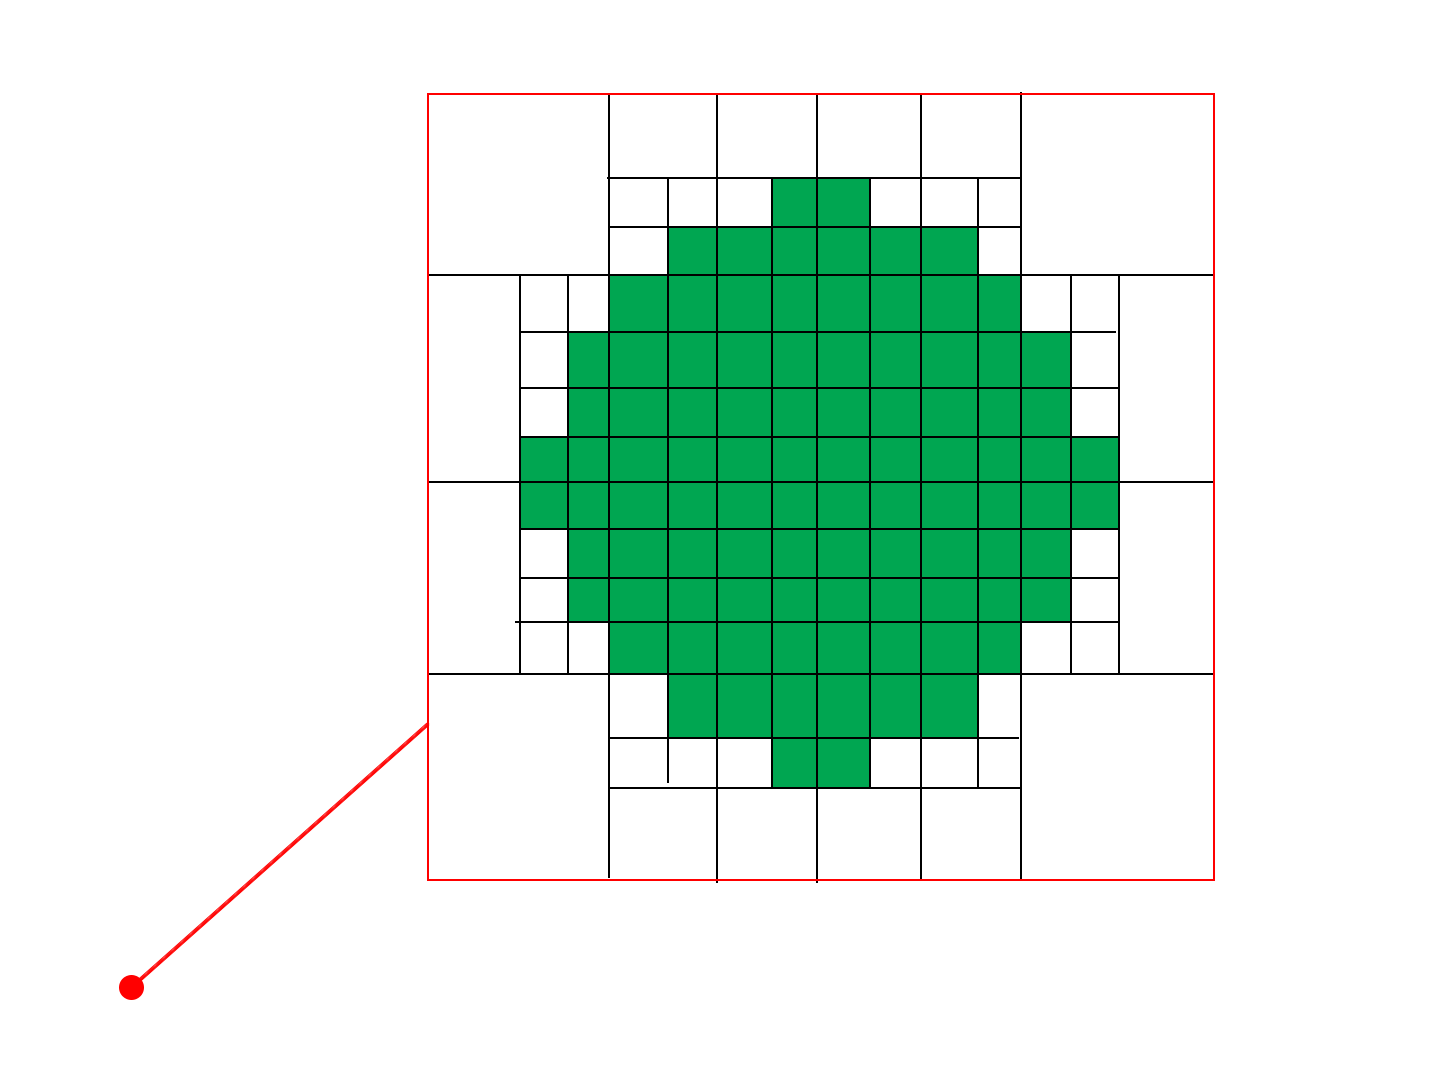
\includegraphics[width=3in]{initial_intersection.png}}
	~
	\subfloat[Initial child selection]{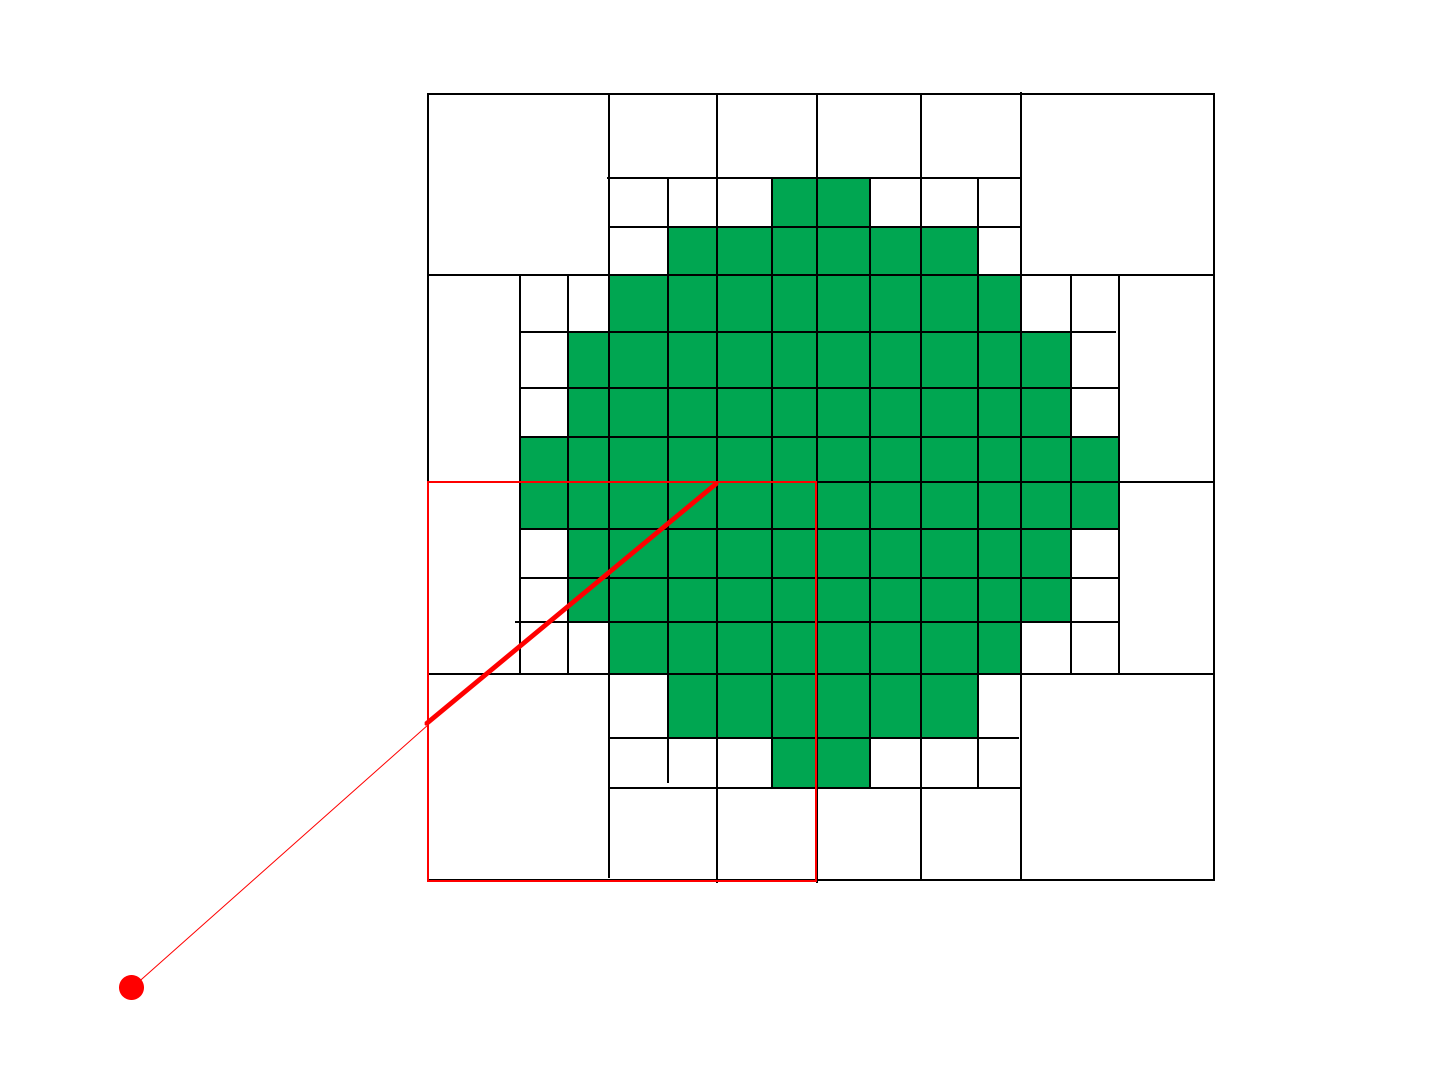
\includegraphics[width=3in]{initial_intersection_child.png}}

	\caption{Initial intersection test}
	\label{fig:root_intersect}
\end{figure}

Pseudo-code for the ray casting algorithm is given in algorithm \ref{alg:raycast}. Our data is stored in a regular octree structure, meaning that each node of the tree is divided into 8 identically sized octants. The algorithm then begins by determining the intersection of the root node with the ray, as well as determining the first entered child octant. This is shown in figure \ref{fig:root_intersect}. The main loop then begins.

\begin{algorithm}
\caption{Ray cast algorithm pseudo-code \parencite{laine10efficientsvos}}
\label{alg:raycast}
\begin{algorithmic}[1]
\Procedure{Raycast}{$root, ray$}
	\State $current\_voxel \gets intersect(root,~ray)$			\Comment{Intersection with root}
	\While{$not~terminated$} \Comment{Traverse}
		\If{$current\_voxel~exists$}
			\If{$voxel~smaller~than~pixel$} 					\Comment{Exit conditions}
				\State $\textbf{return}~current\_voxel$
			\ElsIf{$voxel~is~a~leaf$}
				\State $\textbf{return}~current\_voxel$
			\Else
				\State $current\_voxel \gets push(currrent\_voxel, ray)$		\Comment{Descend into child}
			\EndIf
		\EndIf

		\State $current\_voxel \gets advance(current\_voxel, ray)$			\Comment{Advance into next sibling}

		\If{$advance~direction~disagrees~with~ray~direction$}
			\State $current\_voxel \gets pop(current\_voxel, old\_voxel)$			\Comment{Pop last common parent}
		\EndIf
	\EndWhile
\EndProcedure
\end{algorithmic}
\end{algorithm}

The algorithm then checks that the current voxel exists. If the current voxel exists, the exit conditions are checked: the projection of the current voxel is smaller than the pixel on-screen, and whether the voxel is a leaf node, in which case there are no more subdivisions below it. If either of these conditions are met, the algorithm terminates, returning the current voxel. Otherwise, the algorithm executes push, advancing the traversal to the first entered child voxel.

\begin{figure}
\centering
	\centering
	\subfloat[The current voxel prior to push]{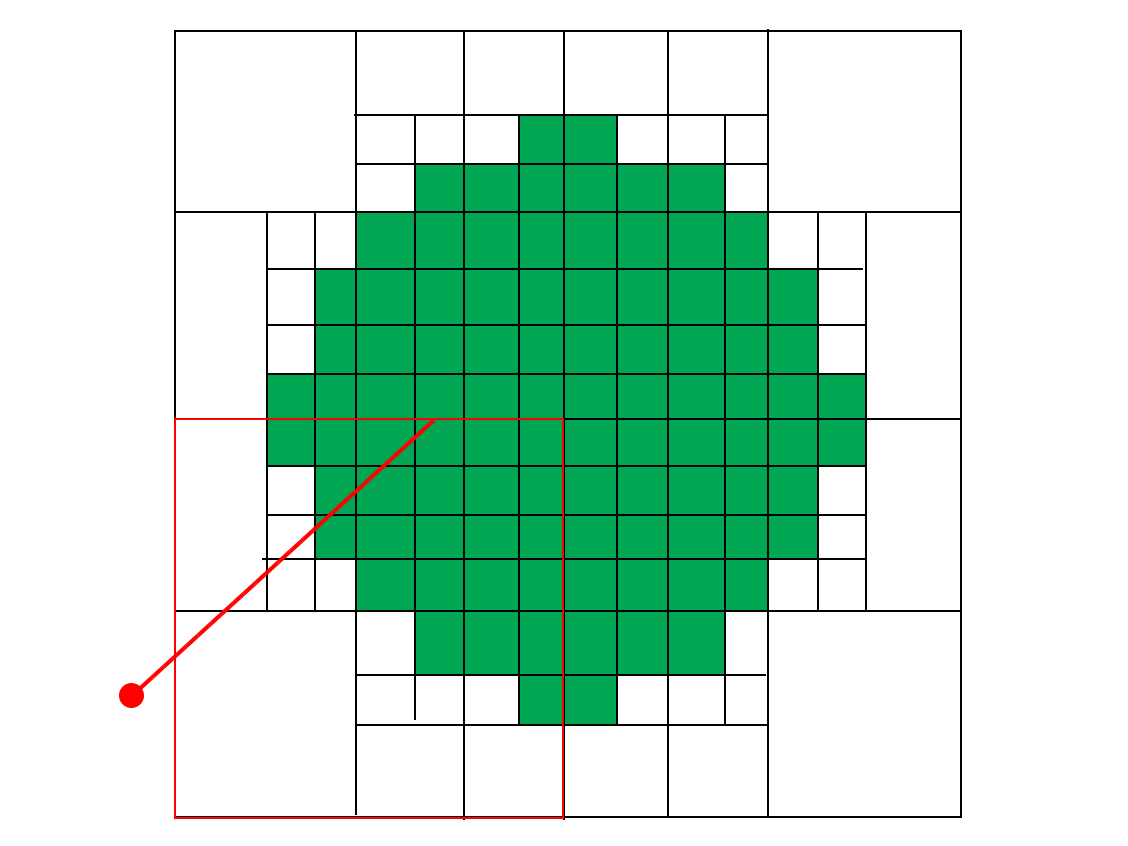
\includegraphics[width=3in]{push_initial.png}}
	~
	\subfloat[The current voxel after push]{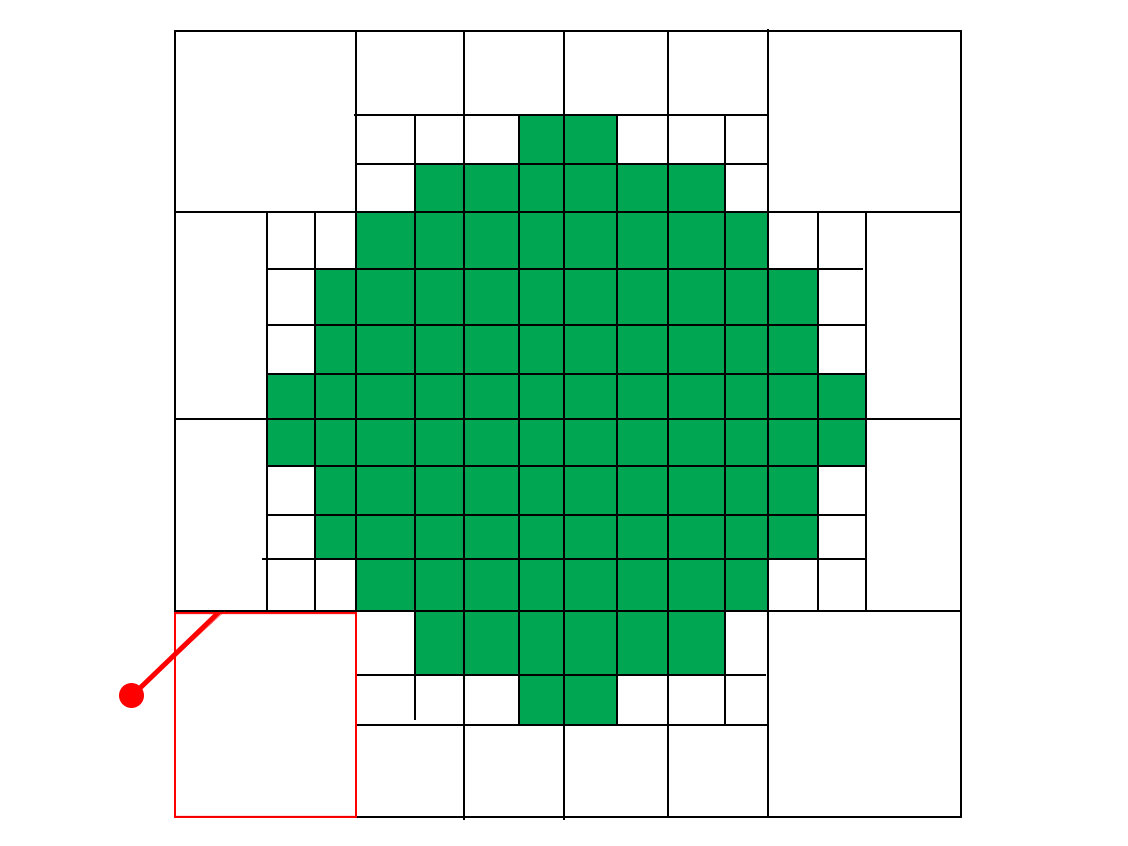
\includegraphics[width=3in]{push_post.png}}

	\caption{The push operation, 2D case}
	\label{fig:ray_push}
\end{figure}

If the current voxel does not exist, the algorithm advances the traversal to the next voxel intersected by the ray on the current level. The direction of advancement is then checked against the ray direction to ensure the advance was valid. If the direction of advance does not coincide with the direction of the ray, in which case one of the parent nodes of the current voxel differs from one of the parent nodes of the previous voxel, pop is used to return to the last common parent of the two voxels and determine the next child intersection along the ray, after which time traversal continues. The push, advance, and pop operations are described fully by \cite{laine10efficientsvos}.

\begin{figure}
\centering
	\subfloat[The current voxel prior to advance]{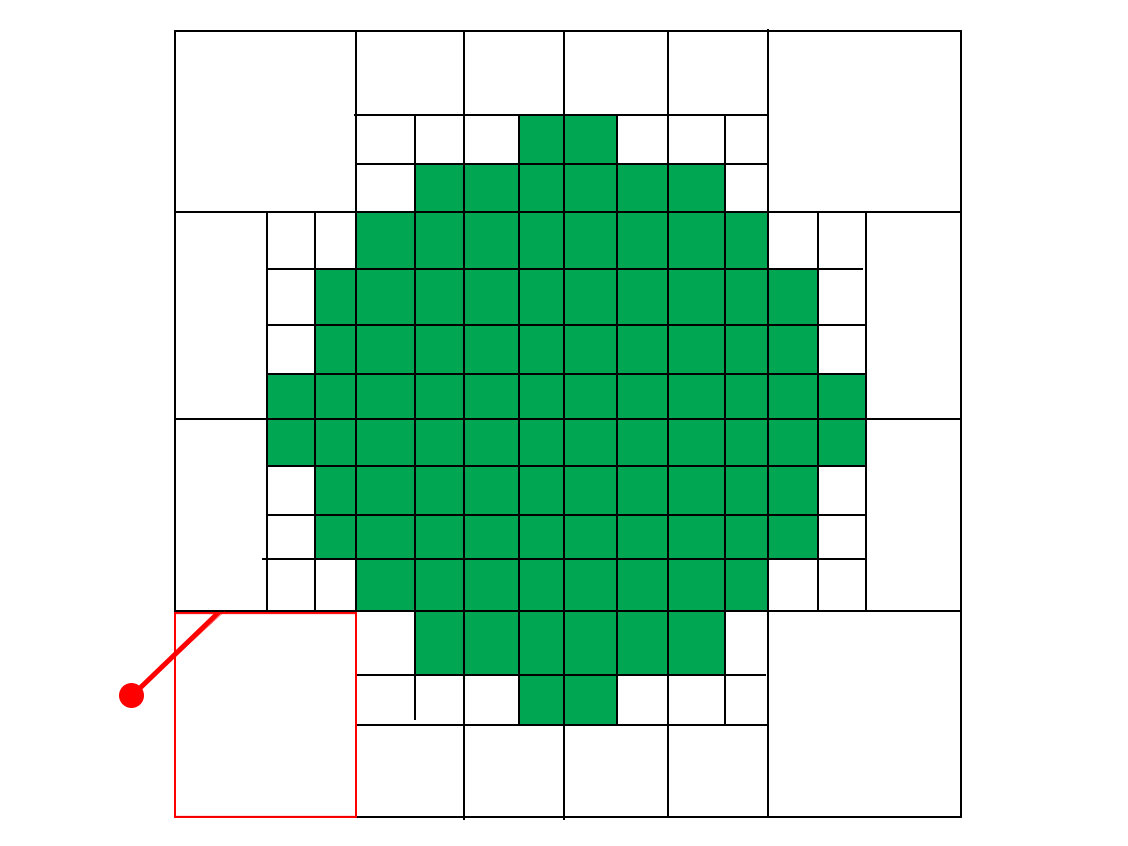
\includegraphics[width=3in]{push_post.png}}
	~
	\subfloat[The current voxel after advance]{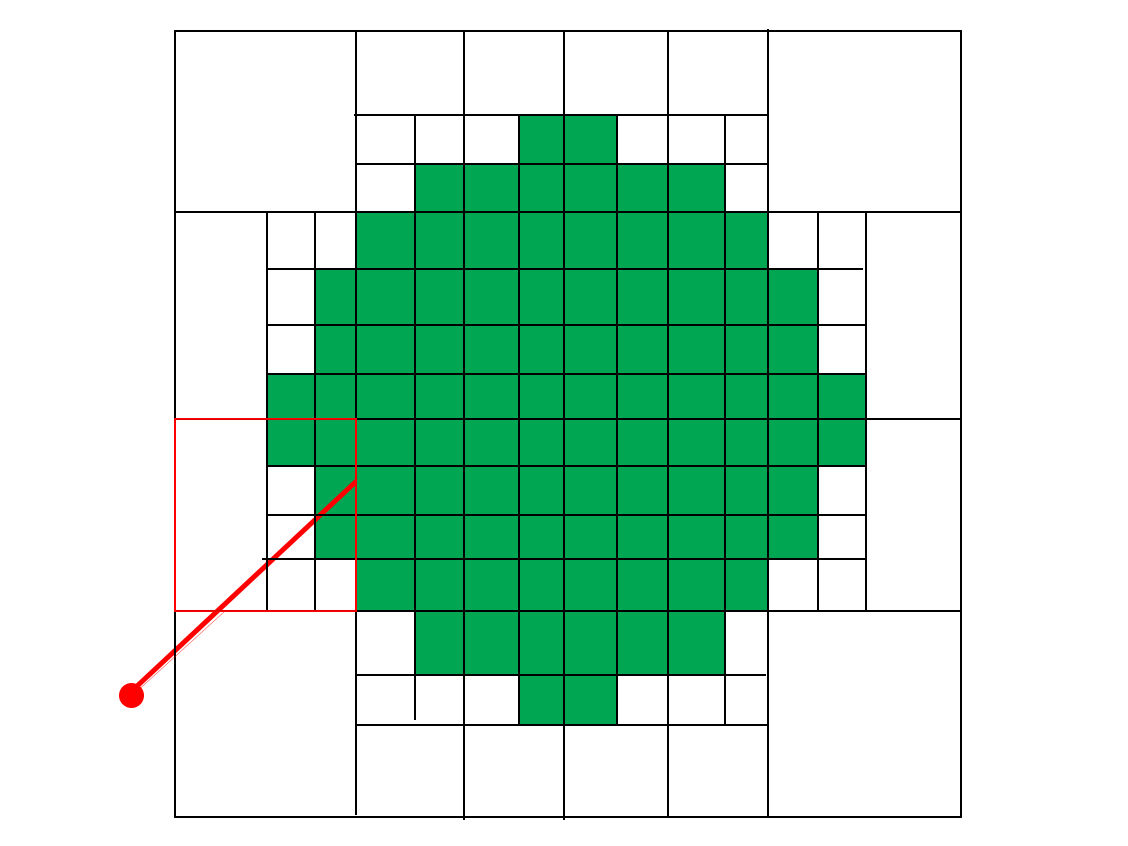
\includegraphics[width=3in]{advance_post.png}}

	\caption{The advance operation, 2D case}
	\label{fig:ray_advance}
\end{figure}

As empty space is quickly advanced over, preventing unnecessary traversal deeper into the tree, and voxels are never revisited, this algorithm quickly determines whether a ray intersects with a volume stored within an octree. This efficient traversal allows us to cast rays against a volume to produce a real-time ray traced image.

\begin{figure}
\centering
	\subfloat[The initially intersected voxel]{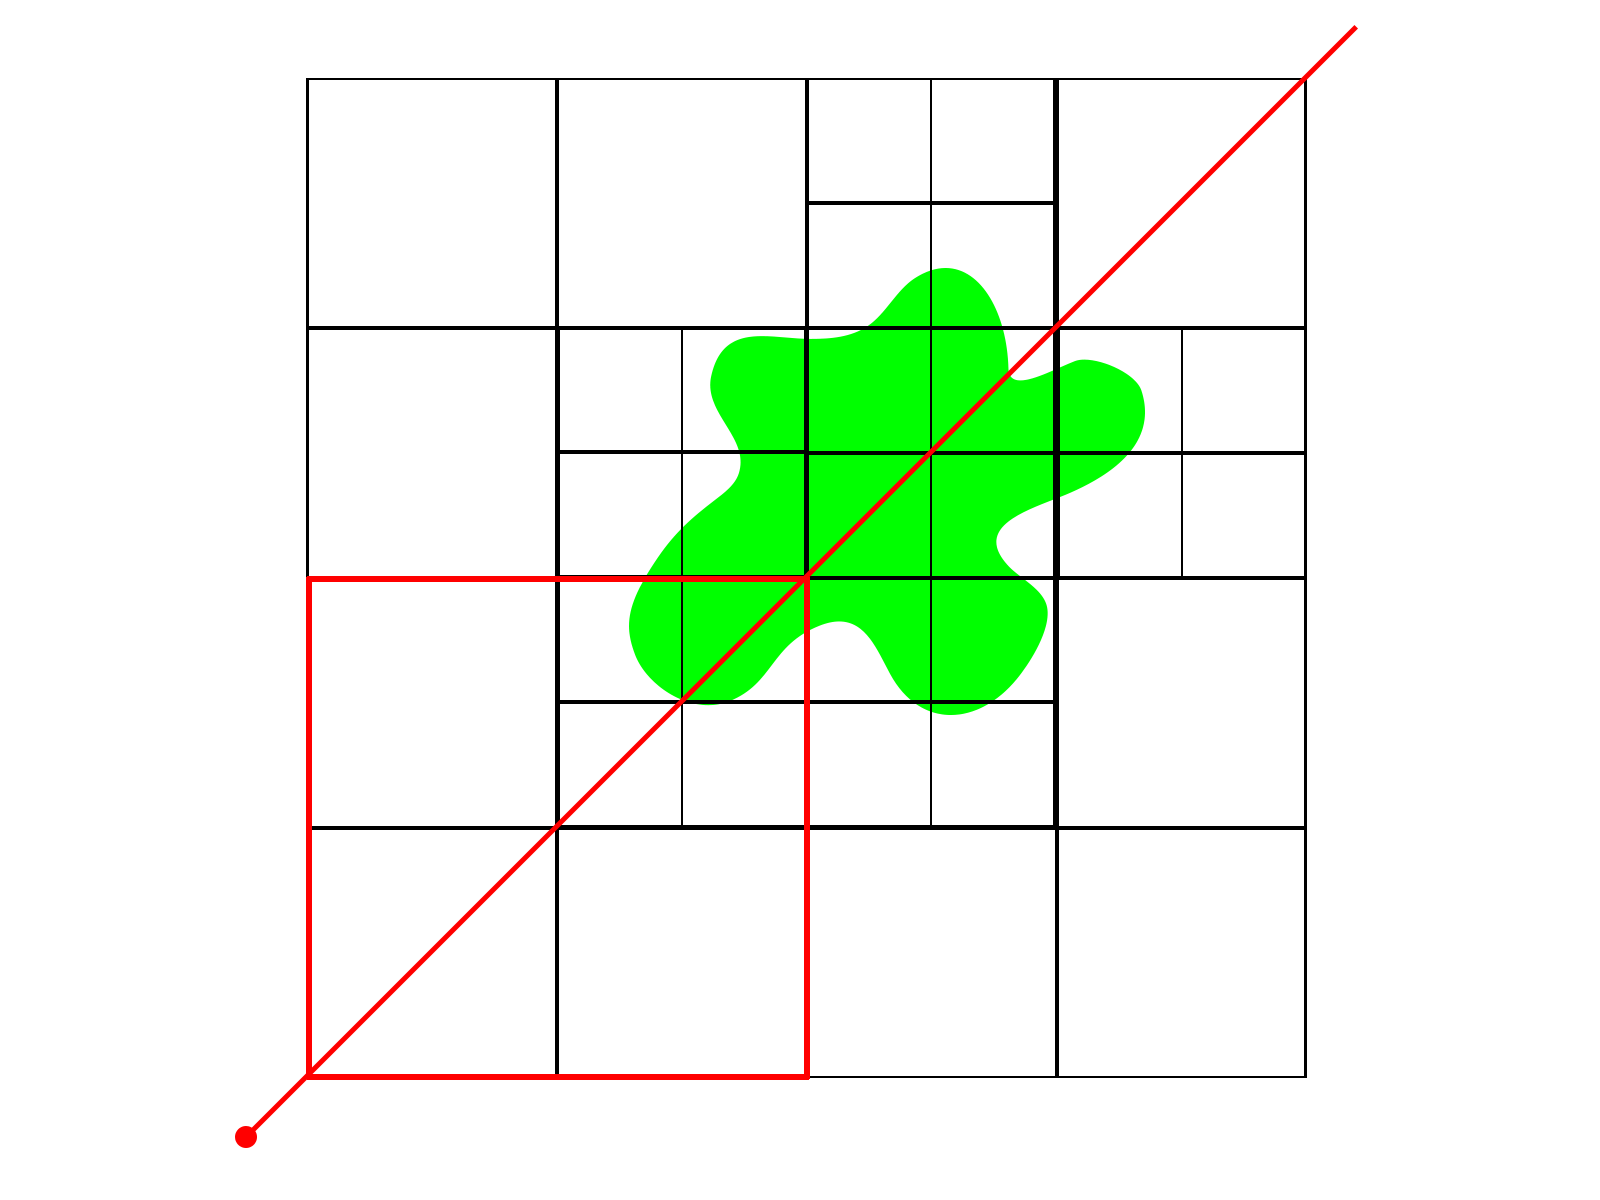
\includegraphics[width=3in]{emptyspace_1.png}}
	~
	\subfloat[Push]{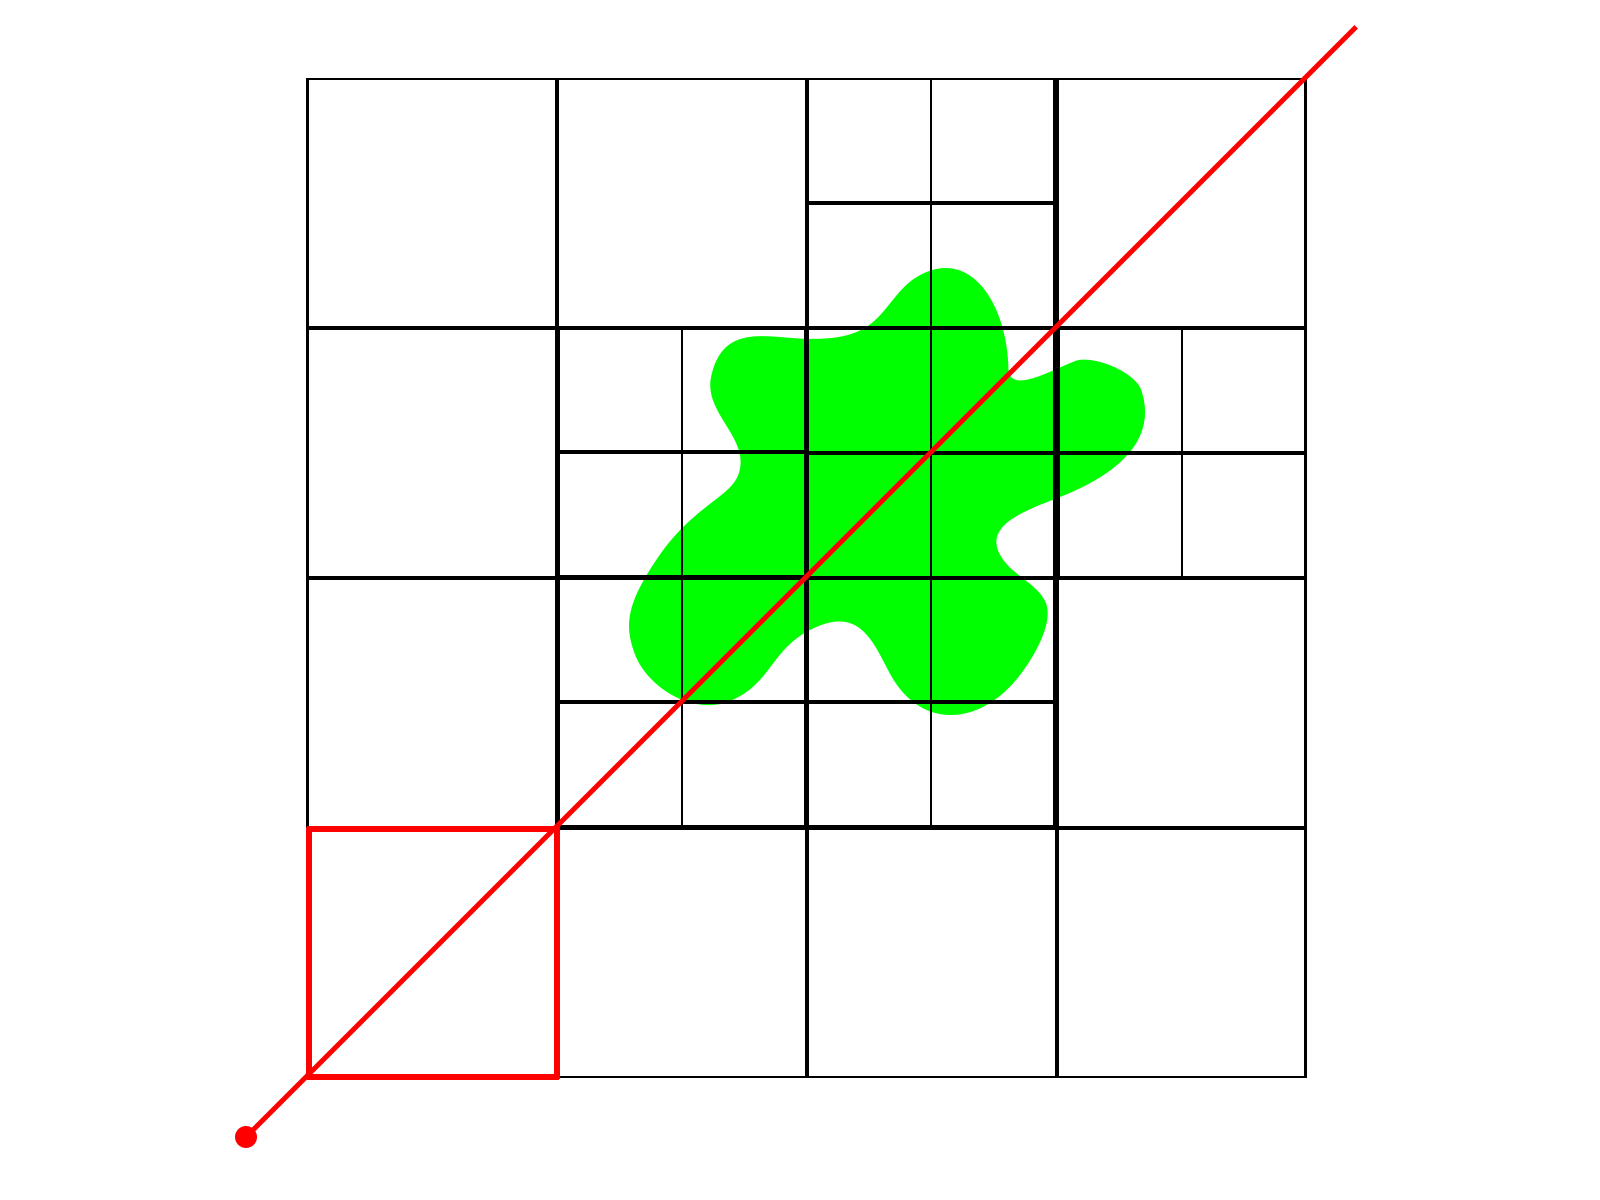
\includegraphics[width=3in]{emptyspace_2.png}}
	\\
	\subfloat[Advance]{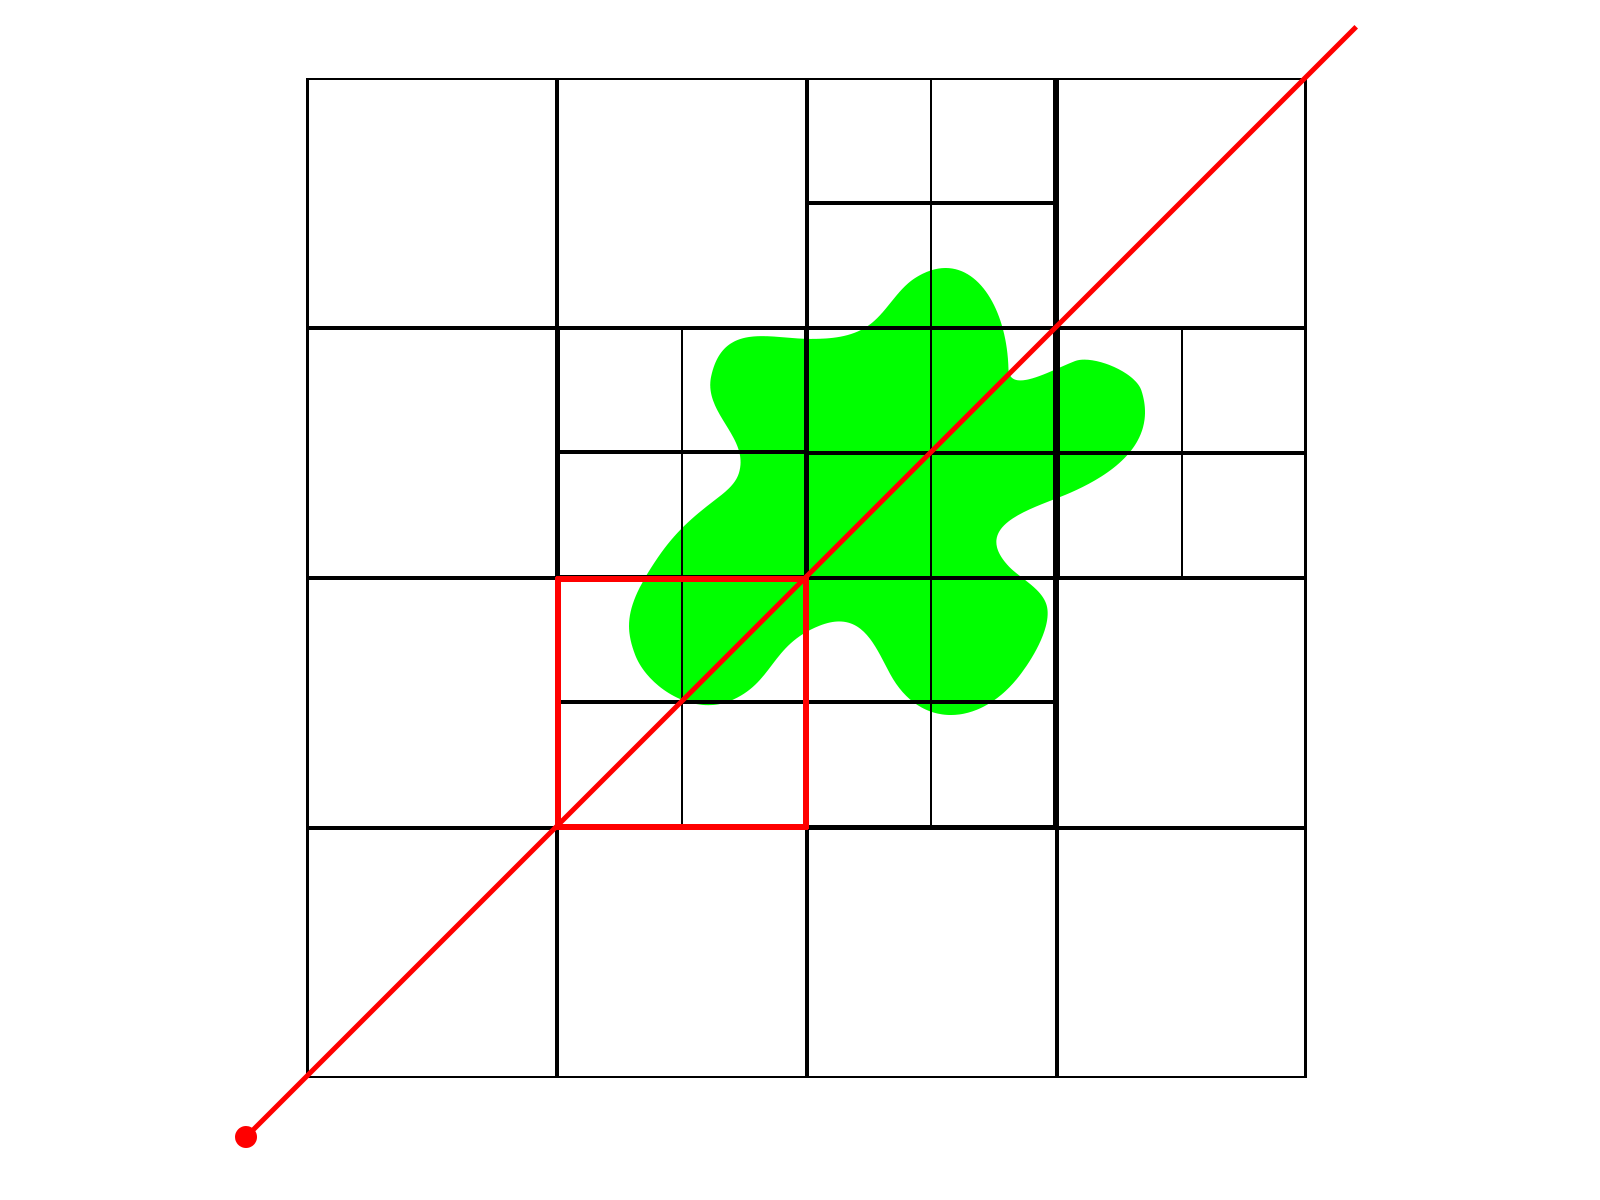
\includegraphics[width=3in]{emptyspace_3.png}}
	~
	\subfloat[Push]{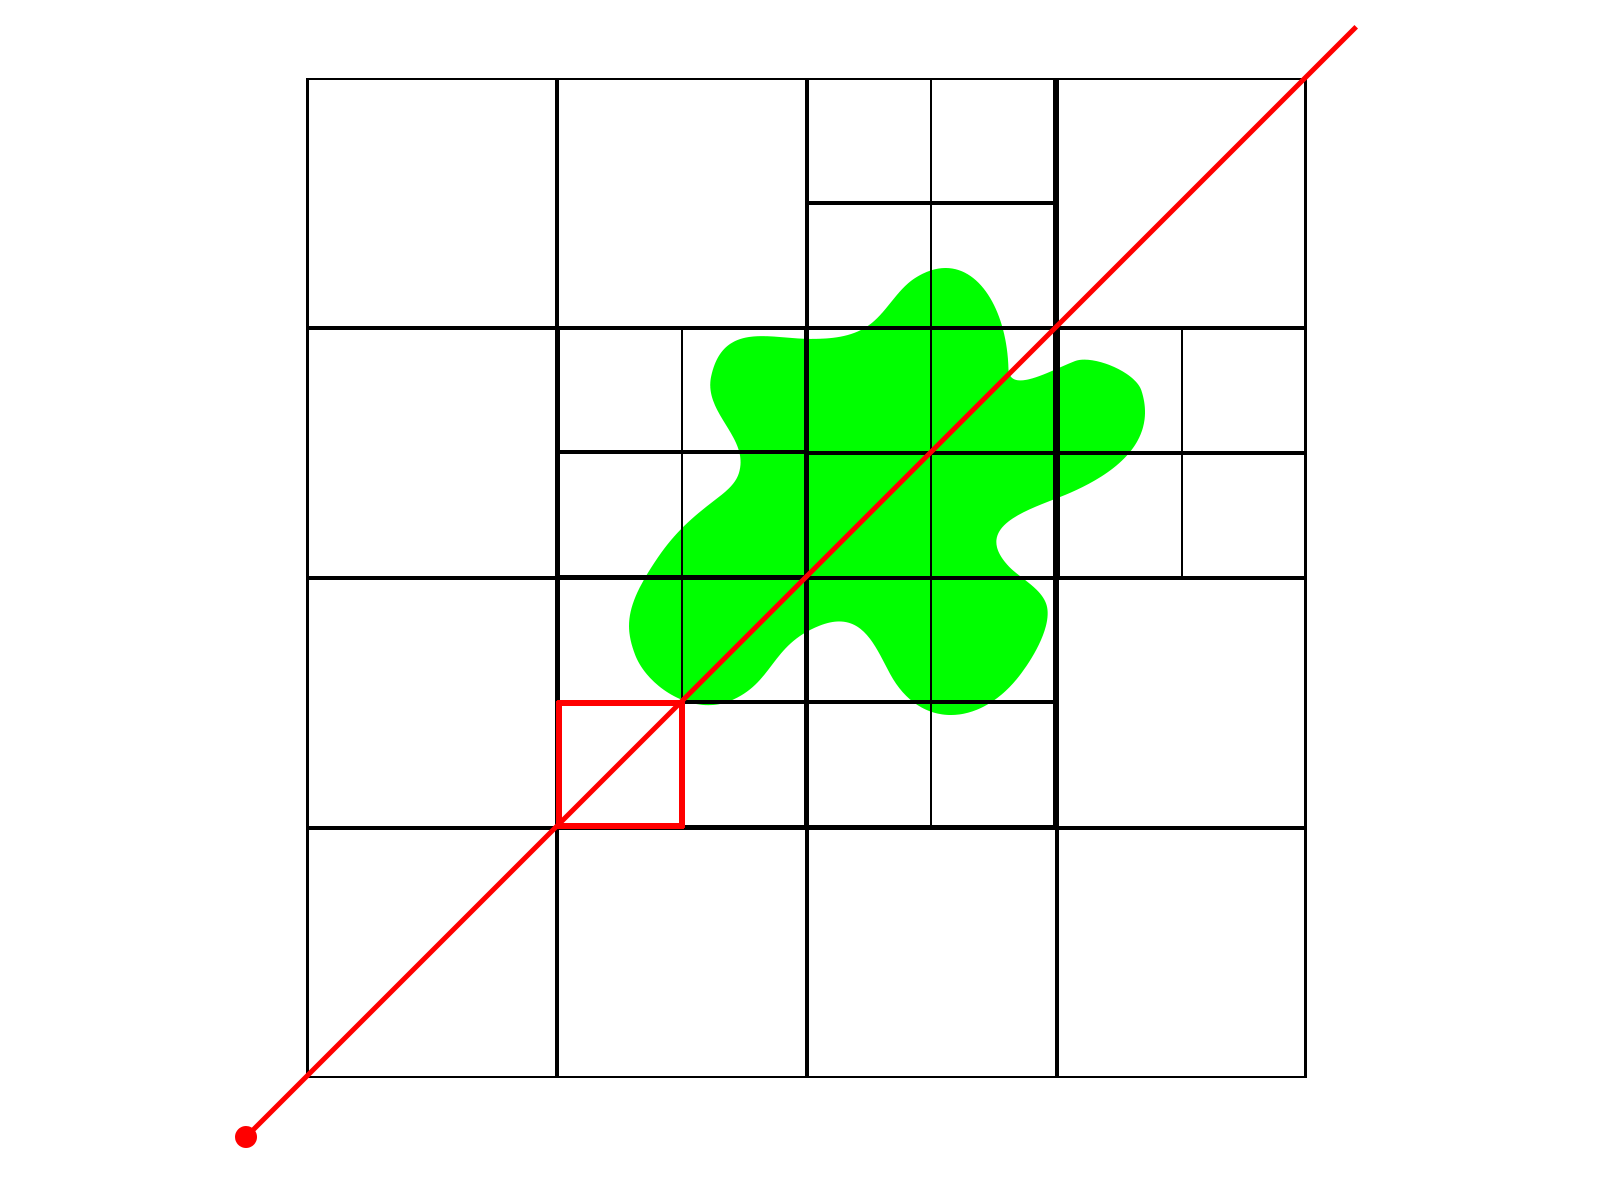
\includegraphics[width=3in]{emptyspace_4.png}}
	\\
	\subfloat[Advance, the first intersected voxel is found]{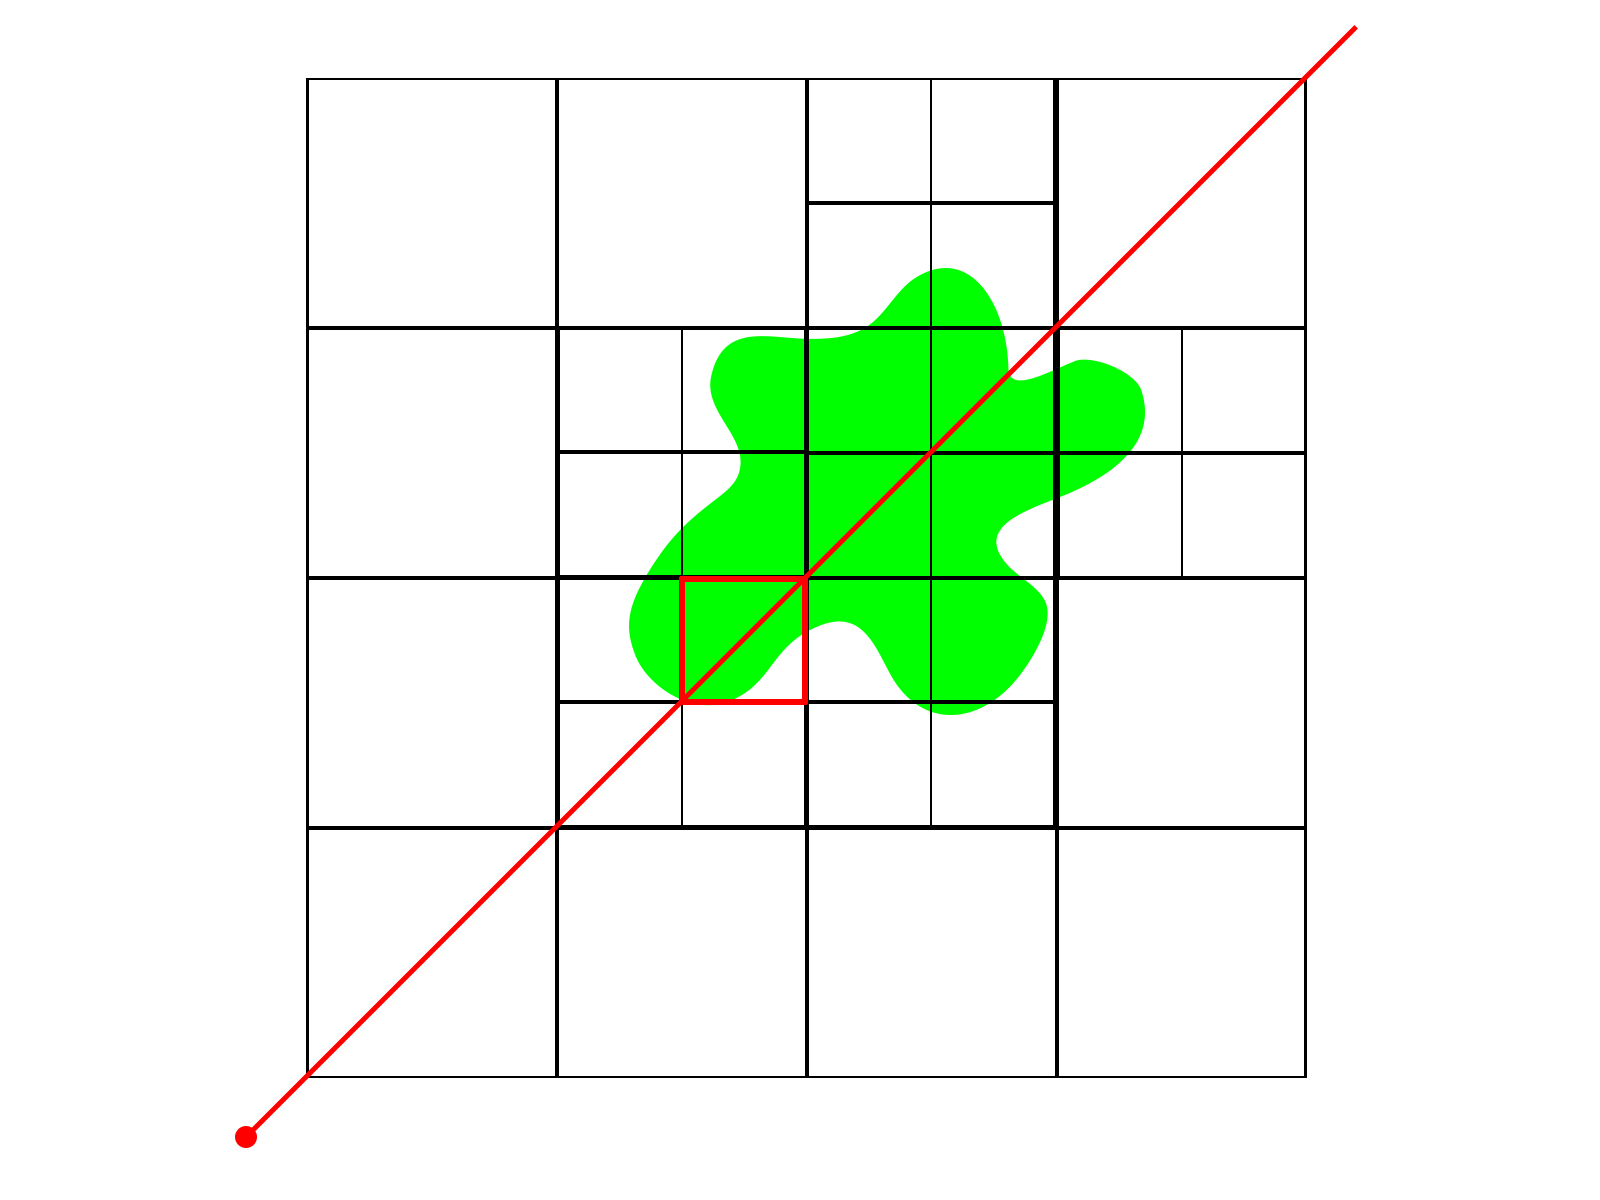
\includegraphics[width=5in]{emptyspace_5.png}}

	\caption{How empty space is avoided, 2D case}
	\label{fig:empty-space}
\end{figure}

\subsection{Storage}
Our data structure uses the same basic storage mechanisms as \cite{laine10efficientsvos}. The tree structure is stored separately from the related shading data, as the majority of processing time is spent in traversal. The extra time it takes to look up shading attributes for shading is therefore traded for a more compact traversal structure. A pointer to a lookup table pointing to attributes for the whole volume is stored at 8 kilobyte boundaries within the tree data.

The tree structure encodes each non-leaf node as a child descriptor, containing a pointer to the children of the current node, an 8-bit mask detailing which of the current node's children exists, and another 8-bit mask which determines which of the node's children are non-leaves (in other words, which children have their own child descriptors stored at the child pointer.)

The child descriptors for the children of a node are then stored together in a block, referenced by this child pointer. The non-leaf mask can then be used to access a particular child using an index from 0 to 7 using a 256 bit lookup table which relates the non-leaf mask of a parent voxel to the index of the desired child:

\[
	child\_offset = lookup(non\_leaf\_mask << child\_index)
\]

The lookup table contains values from 0 to 7, containing the offset of the desired child given a particular non-leaf mask. This lookup table and the relevant implementation is shown in appendix \ref{app:lookup-table}.

\subsubsection{Voxel attributes}
The attributes stored for each voxel are the main way in which our storage scheme varies from that used in \cite{laine10efficientsvos}. In \cite{laine10efficientsvos}, only a colour and a normal, representing the volume after ambient occlusion is pre-calculated, are required for shading. For our purposes, additional attributes are required per-voxel, such as index of refraction and reflectance.

Attributes are stored after the traversal information, along with a lookup table that points to blocks of attributes, grouped by parent voxel. The index in the lookup table can be obtained by considering the offset of the parent's child descriptor from the start of the data, as so:

\[
	lookup\_index = \frac{parent\_desc\_addr - start\_addr}{child\_desc\_size}
\]

The child descriptor size is a constant, referring to the size in bytes of each child descriptor.

This index is then used to retrieve the block of attributes containing the current voxel's attributes, and then the $child\_offset$ obtained above is used to obtain the attributes for the current voxel:

\[
	voxel\_attributes = lookup\_table[lookup\_index] + child\_offset
\]

The resulting pointer points to a structure containing the packed attributes required to shade the current voxel. For our renderer, that includes colour, normal, reflectance, and index of refraction, where the colour also contains an alpha channel which is used to determine transparency. The number of bits used to store each attribute is detailed below:\\

\begin{tabular}{|l|r|l|}
\hline

Attribute & Size in bits & Details \\
\hline

Colour	& 32 bits	& 8 bits for red, green, blue, and alpha components \\
		& 			& between 0.0 and 1.0 \\
\hline

Normal	& 32 bits	& Encoded as detailed in \cite{laine10efficientsvos}, \\
		&			& providing up to 14 bits of precision for smooth \\
		&			& normals \\
\hline

Reflectance & 16 bits & A floating point value between 0.0 and 1.0 \\
\hline

Index of refraction & 16 bits & A floating point value between 1.0 and 4.0 \\
\hline

\end{tabular} \\

The 16-bit floating point values for reflectance are stored as integers between $-2^{15}$ and $2^{15}$, as these are the minimum and maximum values that can be stored in a signed 16-bit integer. These values are scaled such that the minimum value (0.0 for reflectance and 1.0 for refraction) is encoded as $-2^{15}$, and the maximum value as $2^{15}$. Minimum and maximum values were chosen to maximise the precision of the packed values, although the values are packed as 16-bit integers purely for the reason that two 16-bit integers fit exactly into a 32-bit bit-field. If more attributes were added as needed, the sizes of these packed values could potentially be reduced as needed.

The minimum and maximum values for reflectance were chosen as values outside of this range are not physically sensible, as reflectance is defined as the fraction of received electromagnetic radiation (in this case, light) that is reflected by a surface. Values between 0 and 1 for refraction are also not physically sensible, although 4 was chosen as an arbitrary cut-off.

Floating point values are packed into integral bitfields using the following formula, where min and max are the minimum and maximum values to be considered, and bits is the number of bits allocated:

\[	range = max - min \]
\[	int\_max = 1 << (bits - 1) \]
\\
\[	packed\_value = floor((value - min) \cdot \frac{int\_max}{range}) \]

These values are then unpacked as needed. In some cases, this might not be necessary. For example, when checking for changes in index of refraction, the integral value can be used instead.

\section{Reflection rays}
\begin{figure}
\centering
	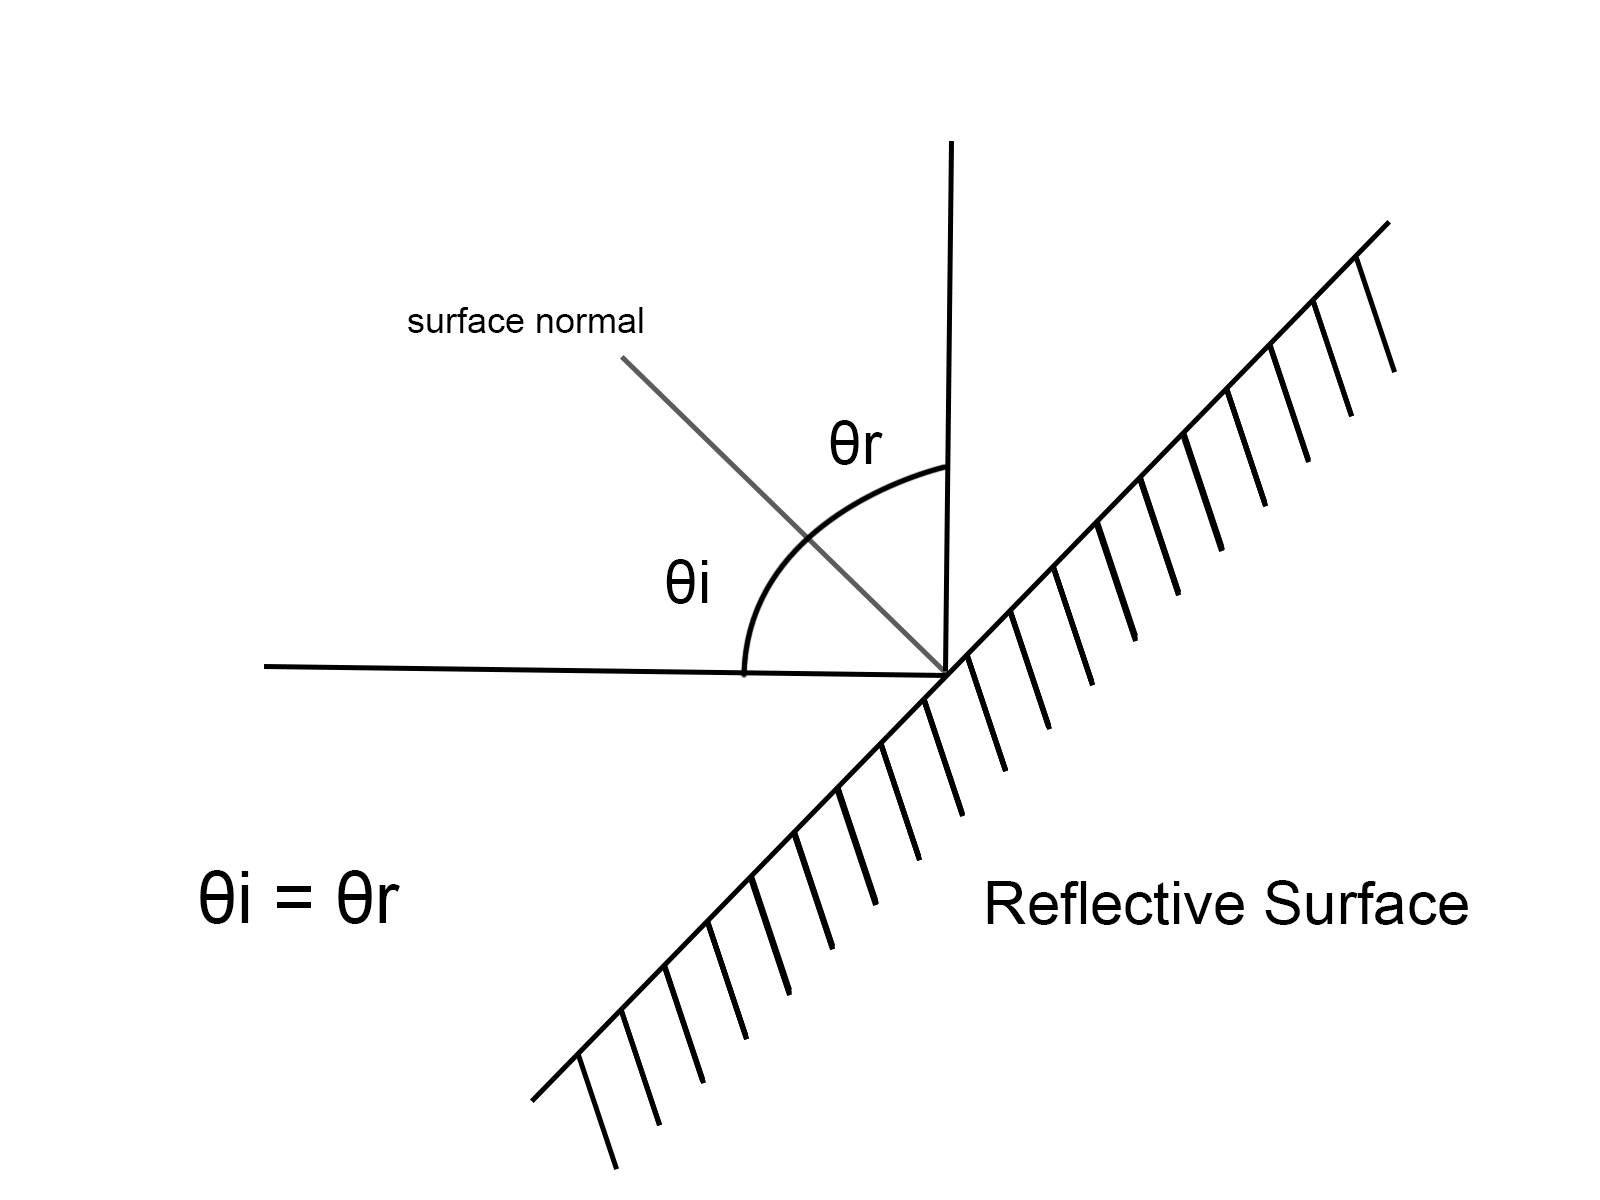
\includegraphics[width=14cm]{reflection.png}
	\caption{The relationship between the angle of incidence $\theta_i$ and the angle of reflection $\theta_r$}
	\label{fig:reflection}
\end{figure}

In order to determine the contribution of light reflected by the scene, a reflection ray must be cast in the angle of reflection in order to find any surfaces that may be reflecting light back. The law of reflection tells us that the angle of incidence, the angle between the normal of a surface and the ray hitting it, is equal to the angle of reflection \parencite{heath99history}. The GLSL (OpenGL Shader Language) specification gives a vector form of this equation using the dot product \parencite{glslspec}, where $I$ is the incident vector and $N$ is the normal of the surface:

\[
	reflection~direction = \vec{I} - 2 * \vec{N} * (\vec{N} \cdot \vec{I})
\]

When shading a surface, a reflection ray is cast in this direction in order to check for intersections with the rest of the scene. If any such intersections are found, the intersected surface is shaded recursively down to a specified limit, and then added onto the overall reflected colour for the current surface.

\section{Refraction rays}
\begin{figure}
\centering
	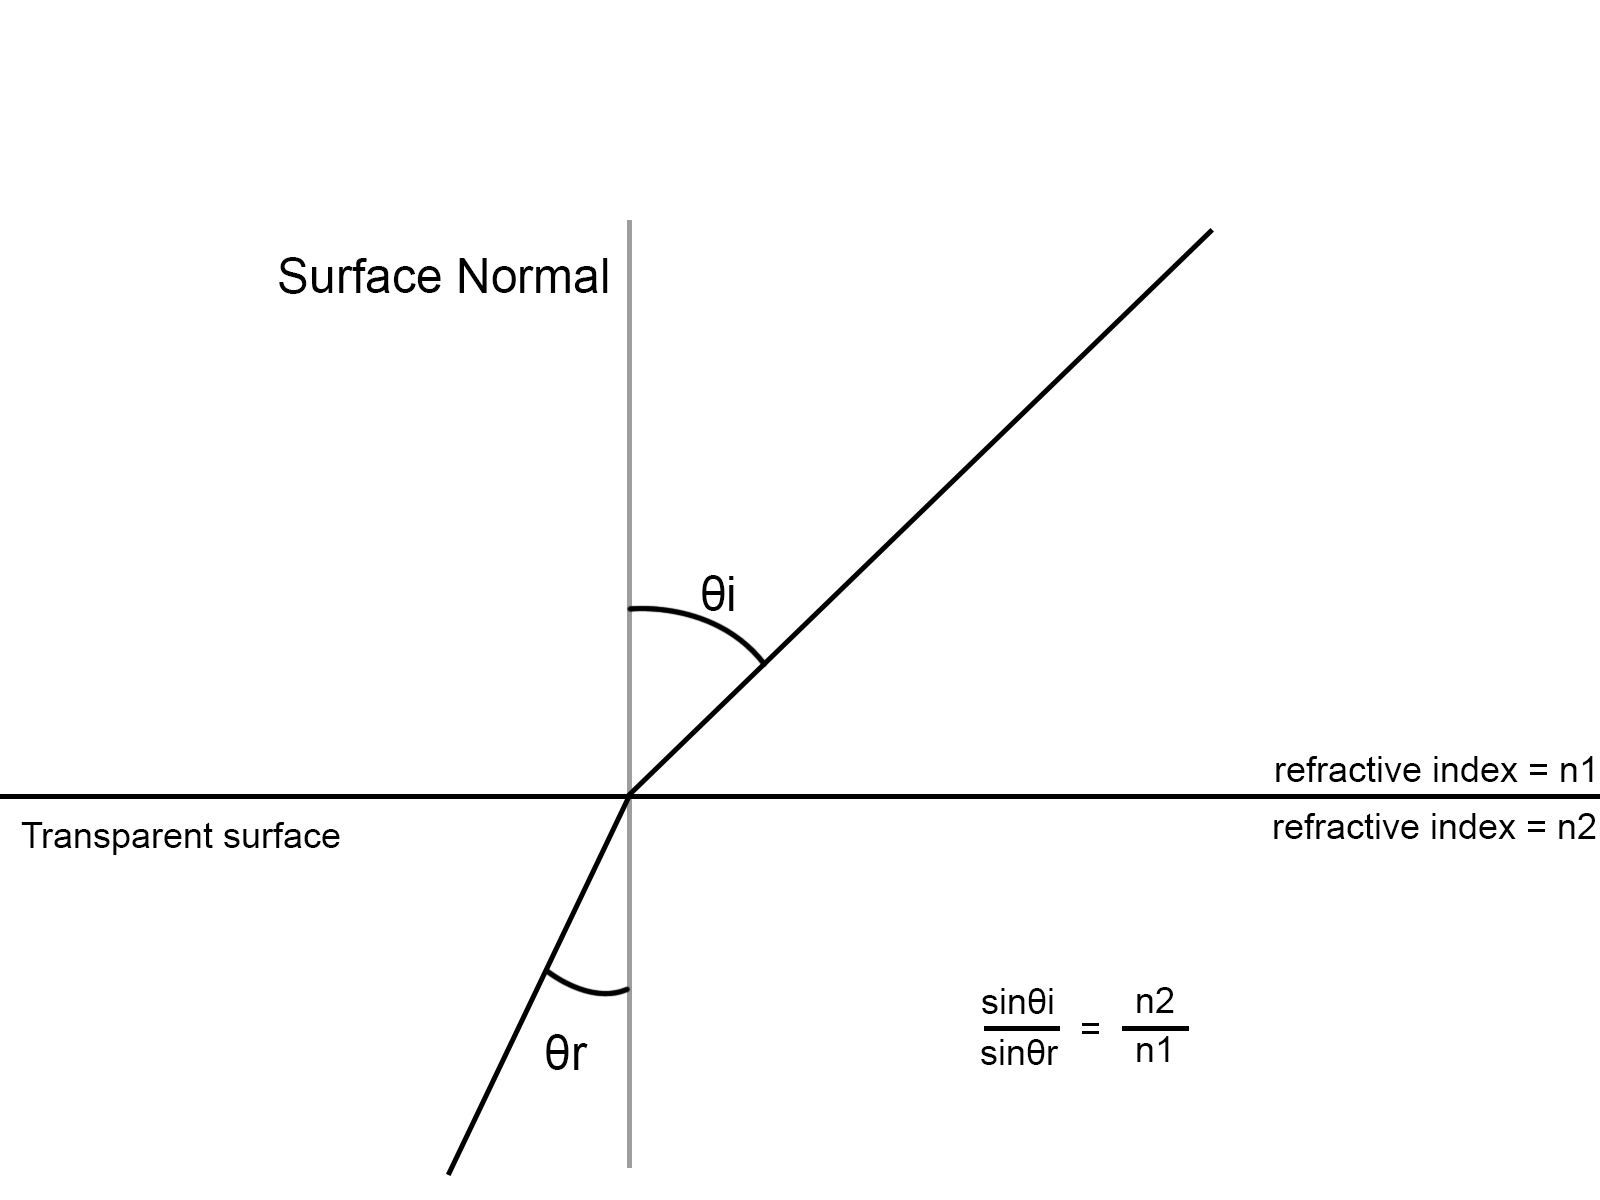
\includegraphics[width=14cm]{refraction.png}
	\caption{The relationship between the angle of incidence $\theta_i$ and the angle of refraction $\theta_r$}
	\label{fig:refraction}
\end{figure}

In order to refract a ray through a surface, the direction of the refracted ray must be calculated. The refracted angle can be calculated by utilising Snell's law, which states a relationship between the angle of incidence $\theta_1$, the angle of refraction $\theta_2$, the index of refraction of the current medium $n1$, and the index of refraction of the medium being entered $n2$ \parencite{glassner89introduction}:

\[
	\frac{\sin\theta_1}{\sin\theta_2} = \frac{n2}{n1}
\]

By using this relationship, it is possible to determine a direction vector for the refracted ray. The GLSL specification again gives a method of calculating a direction vector for a refracted ray, given an incidence vector $I$, a surface normal $N$, and the ratio of the current index of refraction to the new index of refraction $eta$:

\newpage
\lstset{language=C,caption={Calculation of a refraction ray},label=lookuptable}
\begin{lstlisting}[frame=single]
vector refract(vector I, vector N, float eta)
{
	k = 1.0 - eta * eta * (1.0 - dot(N, I) * dot(N, I));

	if (k < 0.0) 
		return vector(0.0, 0.0, 0.0);
	else 
		return eta * I - (eta * dot(N, I) + sqrt(k)) * N;
}
\end{lstlisting}

A refracted ray can then be cast through a material in order to determine the path of light through a medium. When the ray reaches a boundary beyond which the index of refraction changes, the direction of the refraction ray must be recalculated.

One additional consideration must be made, however. The specified normal must be a normal on the plane through which the ray is refracting. In the case of a refraction ray leaving a material, rather than entering it, the normal usually used for rendering a surface will need to be reversed in order to obtain this normal. This can easily be handled by checking the dot product of the normal with the direction of the refracted ray:

\[
	dot = ray.direction \cdot normal
\]

If this dot product is greater than zero, then the surface normal is facing outwards from the direction of the ray, and as such, must be reversed to obtain the normal of the surface through which the ray is being refracted:

\[
	normal = -normal
\]

\subsection{Tracing rays through materials}
In order to handle translucent materials, we must be able to trace a ray through a translucent material. The problem is, given an intersection with a surface, finding the point at which a refraction ray cast from this intersection point exits the surface. One possible solution is to modify the ray casting algorithm, redefining the exit conditions such that it only exits when empty space is found, as in algorithm \ref{alg:raycast_solids}.

\begin{algorithm}
\caption{Ray casting through solids}
\label{alg:raycast_solids}
\begin{algorithmic}[1]
\Procedure{Raycast\_solid}{$root, ray$}
	\State $current\_voxel \gets intersect(root,~ray)$			\Comment{Intersection with root}
	\While{$not~terminated$} \Comment{Traverse}
		\If{$current\_voxel~exists$}
			\State $current\_voxel \gets old\_voxel$
			\State $current\_voxel \gets push(currrent\_voxel, ray)$		\Comment{Descend into child}
		\EndIf

		\State $old\_voxel \gets current\_voxel$
		\State $current\_voxel \gets advance(current\_voxel, ray)$			\Comment{Advance into next sibling}

		\If{$advance~direction~disagrees~with~ray~direction$}
			\State $current\_voxel \gets pop(current\_voxel, old\_voxel)$			\Comment{Pop last common parent}
		\EndIf

		\If{$current\_voxel~nonexistent$}			\Comment{Return when empty space is found}
			\State $\textbf{return}~old\_voxel$
		\EndIf
	\EndWhile
\EndProcedure
\end{algorithmic}
\end{algorithm}

The algorithm will now descend until it finds a leaf node, advancing and popping only once a leaf is found. This algorithm will find the exit point of a ray, but it has the side effect of checking every voxel along the ray's path, at every level. This is very inefficient, and does not take advantage of the volume's tree structure.

On the other hand, if we were to consider the refraction ray discretely, we could follow the path of the ray through the solid, casting back towards the original point of intersection at intervals. Once the active span of the ray as returned by the ray casting algorithm is non-zero, in other words, when the ray has started in empty space and found a surface, we have found the probable exit point of the refraction ray. In order to do this, an interval must be chosen. We chose to use a fixed user-configurable interval, but it may be possible to use a dynamic interval based on the volume being ray traced. The pseudo-code for this operation is given below.

\begin{algorithm}
\caption{Discrete ray cast}
\label{alg:discrete_raycast}
\begin{algorithmic}[1]
\Procedure{Discrete\_raycast}{$root, ray$}
	\State $max\_iterations = \frac{scene\_width}{fixed\_interval}$
	\For{$i = 0;~i<max\_iterations;~++i$}
		\State \Call{Raycast}{origin + i * direction, -direction}
		\If{$resulting~span > 0$} \Comment{We found empty space}
			\State $\textbf{break}$
		\EndIf
	\EndFor
	\State $\textbf{return}~found~surface$
\EndProcedure
\end{algorithmic}
\end{algorithm}

\subsection{Refraction through heterogeneous materials}
It has already been established that the refraction ray's direction must be recalculated when moving from a material with one index of refraction to a material with a different index of refraction. The problem, then, is how to accomplish this for heterogeneous materials.

The above discrete ray cast algorithm can be easily modified to take account of the change in refractive index as it traverses through a material.

\begin{algorithm}
\caption{Discrete ray cast with varying refractive index}
\label{alg:discrete_raycast_heterogeneous}
\begin{algorithmic}[1]
\Procedure{Discrete\_raycast}{$root, ray$}
	\State $max\_iterations = \frac{scene\_width}{fixed\_interval}$
	\State $refractive\_index = hit\_refractive\_index$
	\For{$i = 0;~i<max\_iterations;~++i$}
		\State \Call{Raycast}{origin + i * direction, -direction}
		\If{$resulting~span > 0$} \Comment{We found empty space}
			\State $\textbf{break}$
		\EndIf
		\If{$hit\_refractive\_index != refractive\_index$}
			\If{$\vec{normal} \cdot \vec{direction} > 0$} \Comment{Check if exiting material}
				\State $normal = -normal$
			\EndIf
			\State $direction = \Call{Refract}{direction,~normal,~\frac{refractive\_index}{hit\_refractive\_index}}$
		\EndIf
	\EndFor
	\State $\textbf{return}~found~surface$
\EndProcedure
\end{algorithmic}
\end{algorithm}

\section{Shading}
\begin{figure}
\centering
	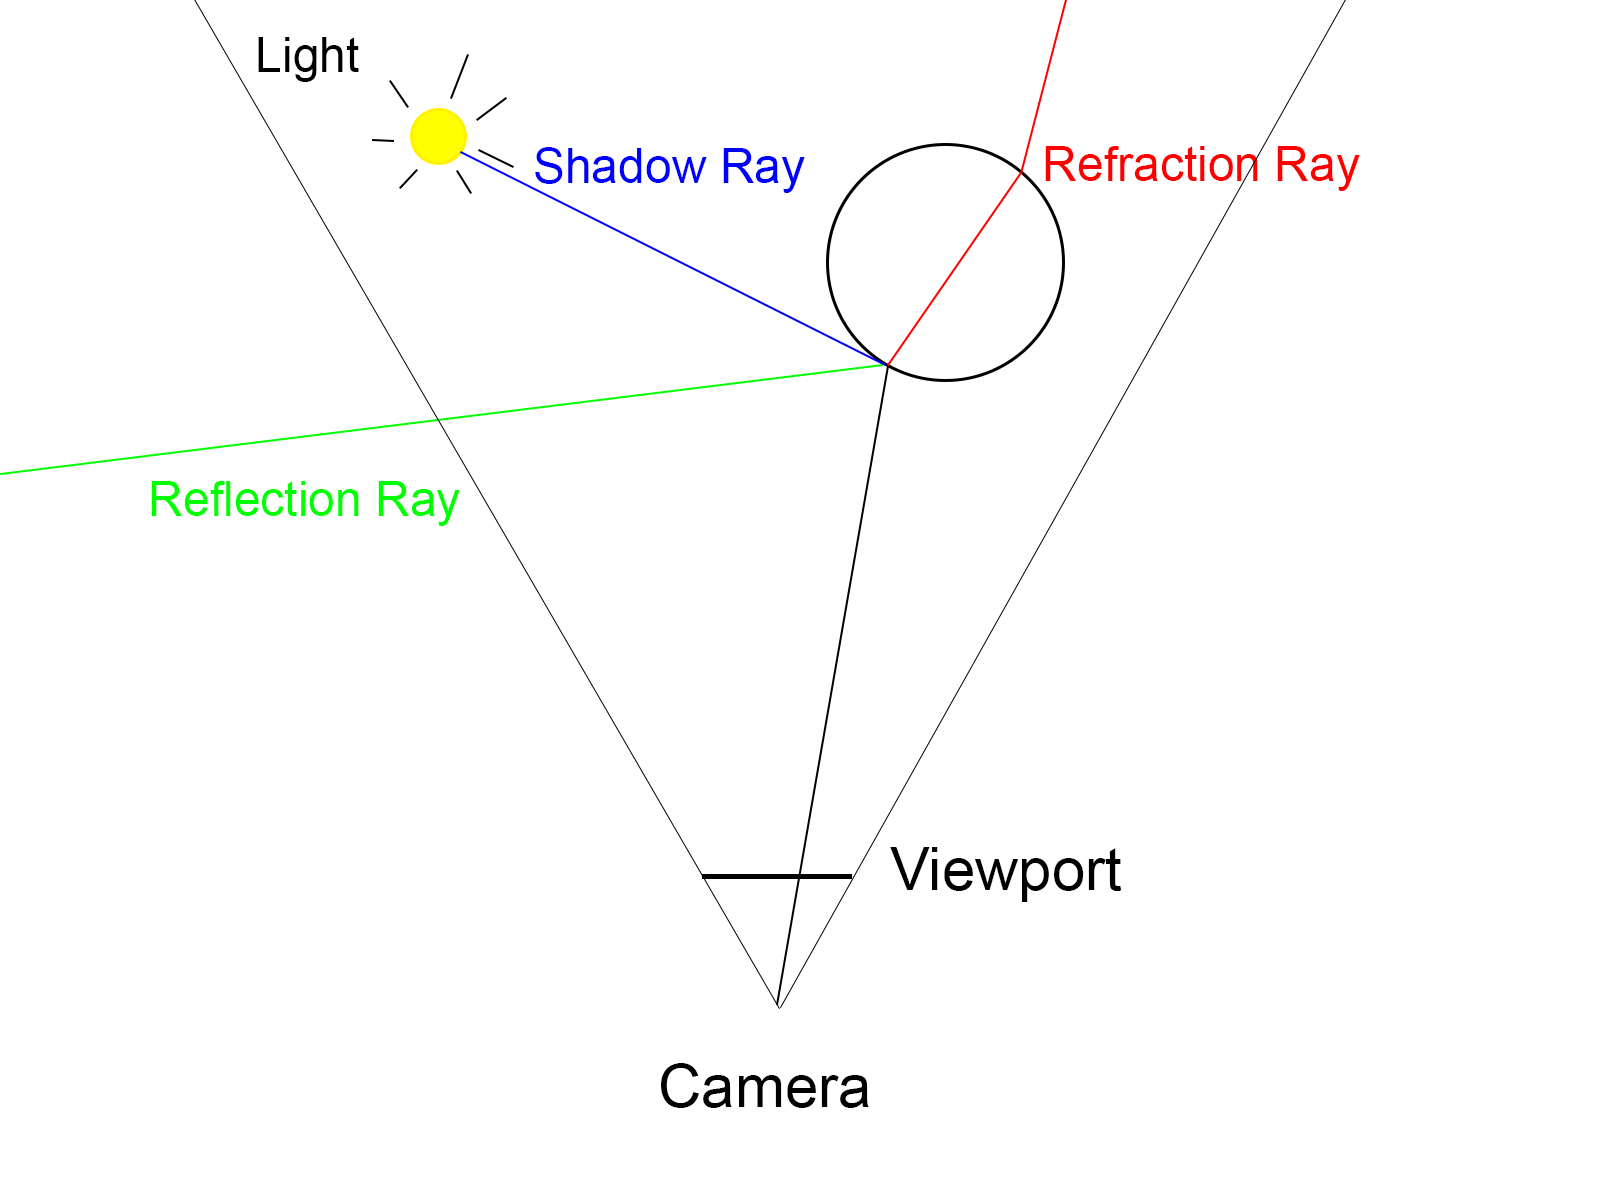
\includegraphics[width=14cm]{secondaryrays.png}
	\caption{Secondary rays being spawned for calculating shadow coverage, reflection, and refraction}
	\label{fig:secondaryrays}
\end{figure}

Our shader uses a Blinn-Phong shading model, as described in chapter \ref{litreview}.

When shading a surface, a ray is cast towards each light source to check if it is occluded, in which case the intersection is in shadow. Reflection and refraction rays are also cast and the results are then mixed additively with the final output colour.

We use recursion to handle multiple levels of reflection and refraction to a predefined maximum. Simplified pseudo-code for rendering and shading is given in algorithm \ref{alg:render}.

\begin{algorithm}
\caption{Per-pixel rendering}
\label{alg:render}
\begin{algorithmic}[1]
\Procedure{render\_pixel}{$x, y, tree, projection$}
	\State $out\_colour \gets (0, 0, 0, 0)$
	\State $ray \gets calculate\_ray(x,~y,~projection)$
	\State $intersection \gets \Call{raycast}{tree, ray}$
	\If{$intersection.hit$}
		\State $out\_colour \gets \Call{shade}{tree,~ ray,~ intersection}$
	\EndIf
	\State $\textbf{return} out_colour$
\EndProcedure
\\
\Procedure{shade}{$tree,~ ray,~ intersection$}
	\State $out\_colour \gets (0, 0, 0, 0)$
	\For{$each~light$} \Comment{Shade for each light}
		\State $light\_dir \gets light\_pos - intersection.position$ \Comment{Check shadow}
		\State $shadow\_ray \gets (intersection.position, light_dir)$
		\State $shadow\_intersection \gets \Call{raycast}{tree, shadow\_ray}$
		\If{$shadow\_intersection.hit$}
			\State $\textbf{continue}$
		\EndIf
		\State $out\_colour ~+=~ \Call{diffuse\_reflection}{intersection,~light}$
		\State $out\_colour ~+=~ \Call{specular\_reflection}{intersection,~light}$
	\EndFor
	\\
	\State $reflection\_ray \gets \Call{reflect}{ray,~intersection}$ \Comment{Reflection}
	\State $reflection\_intersection \gets \Call{raycast}{tree, reflection\_ray}$
	\If{$reflection\_intersection.hit$}
		\State $out\_colour ~+=~ \Call{shade}{tree,~ reflection\_ray,~ reflection\_intersection}$
	\EndIf
	\\
	\State $refraction\_ray \gets \Call{refract}{ray,~intersection}$ \Comment{Refraction}
	\State $refraction\_intersection \gets \Call{raycast\_empty}{tree, refraction\_ray}$
	\If{$refraction\_intersection.hit$}
		\State $out\_colour ~+=~ \Call{shade}{tree,~ refraction\_ray,~ refraction\_intersection}$
	\EndIf
\EndProcedure
\end{algorithmic}
\end{algorithm}

\section{Parallelisation}
Ray tracing is parallelised with one thread per pixel on the screen. This thread is then responsible for the primary ray and all secondary rays, and all work involved in generating that pixel, as shown in algorithm \ref{alg:render}. Pixels are considered independently to allow this process to be parallelised. These threads are spawned on the GPU in 32x32 grids to maximise occupancy. This is the maximum grid size on current generation CUDA GPUs, and allows us to achieve high levels of GPU utilisation as shown in figure \ref{fig:utilisation}.

\begin{figure}
\centering
	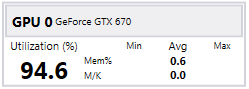
\includegraphics[width=8cm]{gpu0.png}
	\caption{GPU utilisation for our rendering kernel, as determined using Nvidia's nsight profiler}
	\label{fig:utilisation}
\end{figure}

This approach allows us to achieve real-time rendering for simple scenes, and given the results of \cite{laine10efficientsvos} should also allow more complex scenes to be rendered. However, the limitation of this approach is that, as more work is added to each thread, every thread in a grid must follow the most computationally heavy computation path due to the highly parallelised nature of GPUs. Possible solutions to this problem are presented in chapter \ref{conclusion}.

\section{Test data}
Benchmarks for the software were taken by recording the average number of frames per second (FPS) over one minute for a given screen resolution, as well as data resolution. Screen resolution is measured in pixels, while data resolution is measured in nodes of the tree at the lowest level of the tree. This resolution is given by the formula:

\[
	resolution = 2^{max\_scale~ -~ 1}
\]

Such that data generated down to the 11$^{th}$ level has a resolution of $2^{10} = 1024$ in each dimension. This is also referred to as a resolution of $1024^3$.

Each scene has been tested across various screen resolutions as well as data resolutions in order to demonstrate how the algorithms scale with respect to screen ruesolution and data resolution.

In order to evaluate our renderer's performance we have considered the differences in performance for a sample scene with no shadows, reflection or translucency, as screen resolution and data resolution are varied. We consider this data our control sample, and following samples for rendering with shadows, reflection, and translucency is compared with this control.

We have then evaluated the relationships between screen resolution, data resolution, and performance for these samples, as well as compared the overall performance for these samples against our control to determine the effect on performance of considering these effects.

These tests were conducted on a single Nvidia GTX 670.

\section{Implementation}
Our implementation utilises CUDA for all rendering, bypassing the rasterisation process almost entirely. An OpenGL texture is created at program launch, and this texture is then written to by the rendering kernel using OpenGL-CUDA interoperation.

\subsection{OpenGL-CUDA interop}
OpenGL-CUDA interop is accomplished using a pixel buffer object (PBO) that is shared between CUDA and OpenGL. A PBO is stored in GPU memory, eliminating unnecessary copying to main CPU memory. When required by CUDA, the PBO is mapped to a device pointer accessible by cuda, and must be unmapped before it can be accessed again by OpenGL. The PBO can then be unpacked into an OpenGL texture directly, allowing the CUDA-generated buffer to be written to the screen.

A code listing demonstrating how a PBO and a texture are created, and how this PBO is registered with CUDA is available below in code listing \ref{texturecreation}. A code listing for The gpuErrChk macro's code listing is available in appendix \ref{app:cuda-utils}. Once the PBO is created, it can be mapped to a device pointer as shown in code listing \ref{map-buffer}. Once unmapped, its contents can then be unpacked to a texture for display on the screen as demonstrated in \ref{pbo-unpack}. As all of these operations occur directly within GPU memory, unnecessary coping to main memory is avoided.

\subsection{Matrix maths}
Matrix maths is accomplished using GLM, the OpenGL Mathematics library. This is a C++ library which implements all of the features of GLSL and includes CUDA support, making it suitable for writing 3D rendering code and shaders in CUDA.

\newpage
\lstset{language=C,caption={Creation of the OpenGL PBO and texturre},label=texturecreation}
\begin{lstlisting}[frame=single]
void* glFb;

GLuint pbo;
GLuint texid;

// Create pixel buffer object
glGenBuffers(1, &fbo);

// Create buffer texture
glGenTextures(1, &texid);

// Initilaise pixel buffer object with size
glBindBuffer(GL_PIXEL_UNPACK_BUFFER, pbo);
glBufferData(GL_PIXEL_UNPACK_BUFFER,
	viewport.w * viewport.h * 4 * sizeof(GLubyte),
	nullptr, GL_DYNAMIC_DRAW);
glBindBuffer(GL_PIXEL_UNPACK_BUFFER, 0);

// Initialise texture with width, height, and format
glBindTexture(GL_TEXTURE_2D, texid);
glTexImage2D(GL_TEXTURE_2D, 0, GL_RGBA, width, height, 0,
				GL_RGBA, GL_UNSIGNED_BYTE, NULL);
glTexParameteri(GL_TEXTURE_2D, GL_TEXTURE_MAG_FILTER, GL_LINEAR);
glTexParameteri(GL_TEXTURE_2D, GL_TEXTURE_MIN_FILTER, GL_LINEAR);
glBindTexture(GL_TEXTURE_2D, 0);

// Register pixel buffer object with cuda
gpuErrchk(cudaGraphicsGLRegisterBuffer(&glFb, pbo,
			cudaGraphicsRegisterFlagsNone));
\end{lstlisting}

\newpage
\lstset{language=C,caption={Binding the PBO so that CUDA kernels can access it},label=map-buffer}
\begin{lstlisting}[frame=single]

// Bind cuda graphics resources
gpuErrchk(cudaGraphicsMapResources(1, &glFb, 0));

// Get a device pointer to it
gpuErrchk(cudaGraphicsResourceGetMappedPointer(&ptr, &size,
												glFb));

// Pass device pointer to CUDA kernel

// Unmap pbo
gpuErrchk(cudaGraphicsUnmapResources(1, &glFb, 0));
\end{lstlisting}

\lstset{language=C,caption={Unpacking of a PBO to an OpenGL texture},label=pbo-unpack}
\begin{lstlisting}[frame=single]
glBindBuffer(GL_PIXEL_UNPACK_BUFFER, pbo);
glBindTexture(GL_TEXTURE_2D, texid);
glTexEnvi(GL_TEXTURE_ENV, GL_TEXTURE_ENV_MODE, GL_REPLACE);
glTexImage2D(GL_TEXTURE_2D, 0, GL_RGBA, width, height, 0,
				GL_RGBA, GL_UNSIGNED_BYTE, 0);
\end{lstlisting}		% 15%
\chapter{Implementation}
\label{implementation}

\section{Ray-casting}

\subsection{Contours}

\section{Ray-tracing}

\section{Shading}

\section{Data structure}

\subsection{Generation}

\subsubsection{Sphere}

\subsubsection{Mesh}			% }
\chapter{Combining Approaches}
\label{combining}		% } 15%
\chapter{Realtime Effects}
\label{realtime-effects}			% }
\chapter{Rendering Multiple Objects}
\label{combining}			% }
\chapter{Results and Analysis}
\label{results}		% 20%
\chapter{Evaluation}
\label{evaluation}				%
\chapter{Future Work}
\label{future_work}				%
\chapter{Conclusion}
\label{conclusion}				% 15%

% Bibliography TOC entry
\cleardoublepage
\phantomsection
\addcontentsline{toc}{chapter}{Bibliography}

% Show bibliography
\nocite{*}
\printbibliography

% Appendices TOC entry
\cleardoublepage
\phantomsection
\addcontentsline{toc}{chapter}{Appendices}

% Use letters for appendix sections and numbers for subsections
\renewcommand\thesection{\Alph{section}}
\renewcommand\thesubsection{\arabic{subsection}}

% Remove individual appendices from TOC
\addtocontents{toc}{\setcounter{tocdepth}{-1}}

% Include appendicies
\appendix
\section{Source code}

\subsection{Hello, world!}

\lstset{language=C++}
\begin{lstlisting}
int main(int argc, char** argv)
{
	printf("Hello, world!");
}
\end{lstlisting}

\end{document}

